\documentclass[9pt]{beamer}
\usepackage[utf8]{inputenc}
\usepackage[czech]{babel}
\usepackage{graphicx}
\usepackage{pifont}
\usepackage{listings}

\beamertemplatenavigationsymbolsempty

\graphicspath{ {resources/} }

\usetheme{Madrid}
\usecolortheme{seagull}

\title{Maturitní projekt}
\author{Jakub Rada O8.B}
\institute{Gymnázium Nad Alejí}
\date{28.02.2019}

\begin{document}
    \frame{\titlepage}
    \begin{frame}
        \frametitle{O aplikaci}
        Aplikace na vytváření, úpravy a učení se slovíček nebo jiné látky
        \begin{itemize}
            \item<1-> vytváření kartiček \ding{219} dvojice slov / vět
            \item<1-> vytváření okruhů (tagů), do kterých lze přidávat kartičky
            \item<1-> 3 typy testů
            \begin{enumerate}
                \item<1-> procházení kartiček bez zadávání odpovědi
                \item<1-> vybírání z možností
                \item<1-> psaní správné odpovědi
            \end{enumerate}
            \item<1-> import, export kartiček a okruhů
        \end{itemize}
    \end{frame}
    \begin{frame}
        \frametitle{Použité jazyky}
        \begin{itemize}
            \item<1-> Python Django
            \item<1-> Html, Css (Bootstrap)
            \item<1-> Javascript
            \item<1-> Electron
        \end{itemize}
        \begin{figure}
            \centering
            
\includegraphics[width=0.6\linewidth]{logos.jpg}
        \end{figure}
    \end{frame}
    \begin{frame}
        \frametitle{Problémy a úspěchy}
        \textbf{Problémy}
        \begin{itemize}
            \item odpovědi z databáze nepřichází ve stejném pořadí jako odešly
            \begin{itemize}
                \item každá \textit{query} trvá jinak dlouho
                \item při testech lepší, problém při řazení položek v seznamu
            \end{itemize}
            \item test vybírání z možností při malém počtu kartiček ($< 4$)
            \begin{itemize}
                \item nesprávné odpovědi se vybírají z daného okruhu (1 kartička v okruhu \ding{219} ve výběru je pouze 1 možnost)
            \end{itemize}
        \end{itemize}
        \textbf{Úspěchy}
        \begin{itemize}
            \item porovnávání odpovědí při psacím testu
            \begin{itemize}
                \item implementace \textit{Levenshteinovy vzdálenosti}
            \end{itemize}
            \item kartičky se stejnou jednou stranou (jedno slovíčko má více překladů)
            \begin{itemize}
                \item stejná přední strana \ding{219} odpovědi se spojí do jedné
                \item stejná zadní strana \ding{219} automaticky se vygeneruje jiná odpověď
            \end{itemize}
        \end{itemize}
    \end{frame}
    \begin{frame}
        \frametitle{Import a export}
        Import i export ve formátu \texttt{.yml}
        \begin{figure}
            \centering
            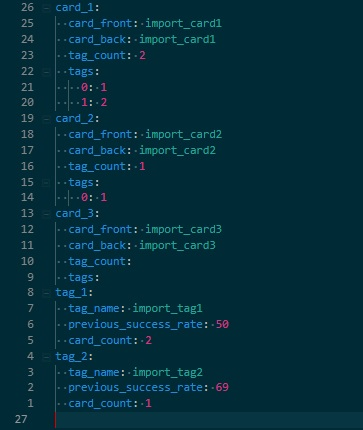
\includegraphics[width=0.5\linewidth]{yml_example.jpg}
        \end{figure}
    \end{frame}
    \begin{frame}
        \frametitle{Ukázka}
    \end{frame}
    \begin{frame}
        \frametitle{Další vylepšení}
        \begin{itemize}
            \item<1-> Změnit barvy
            \item<1-> Řazení kartiček podle názvu
            \begin{itemize}
                \item<1-> Seřazený list se netiskne správně
            \end{itemize}
            \item<1-> Vylepšit hodnocení správnosti
            \begin{itemize}
                \item<1-> Zatím stačí mít 1/2 slova správně
            \end{itemize}
            \item<1-> Opravit zvýrazňování chyb u kratších slov než je správná odpověď
        \end{itemize}
        \begin{columns}
            \column{0.5\linewidth}
            \begin{figure}
                \centering
                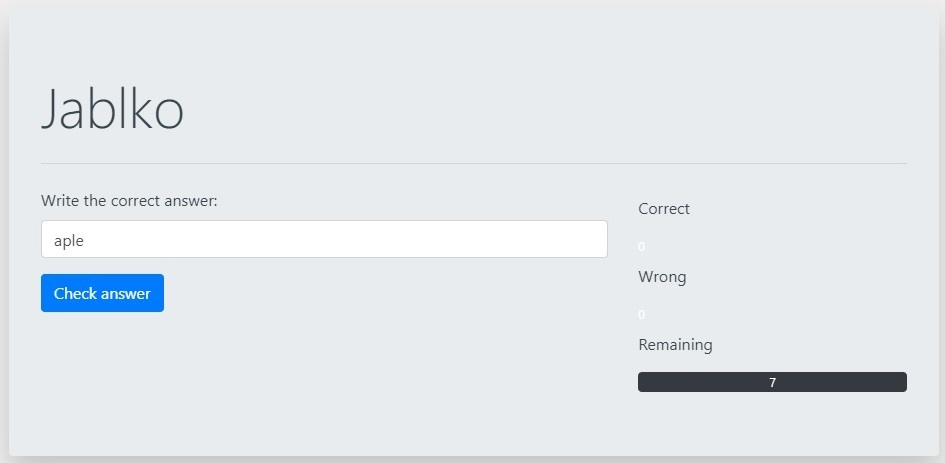
\includegraphics[width=\linewidth]{highlight-error_1.jpg}
            \end{figure}
            \column{0.5\linewidth}
            \begin{figure}
                \centering
                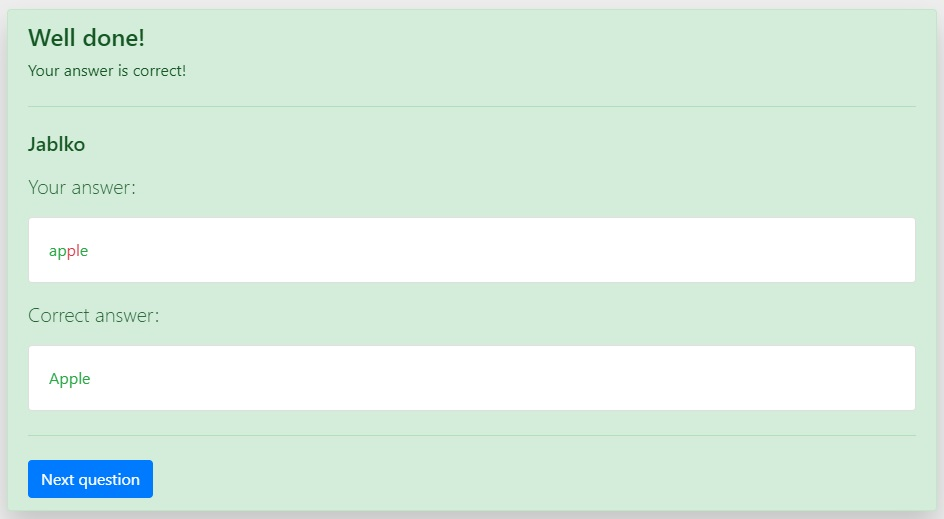
\includegraphics[width=\linewidth]{highlight-error_2.jpg}
            \end{figure}
        \end{columns}
        \begin{itemize}
            \item<1-> Název, titulní strana, dokumentace a nápověda
        \end{itemize}
    \end{frame}
    \begin{frame}
        \begin{block}{}
            \centering
            {\Huge Děkuji za pozornost}
        \end{block}
    \end{frame}
\end{document}